
\documentclass[crop,tikz]{standalone}
\usepackage[english]{babel}
\usepackage{amsmath,amssymb}
\usepackage{bbm}
\usepackage{graphicx}
\usepackage{tikz}
\usepackage{xcolor}
\usepackage{caption}
\usepackage{subcaption}

\usetikzlibrary{arrows, positioning, shapes, fit}

\definecolor{tabblue}{HTML}{1f77b4}
\definecolor{taborange}{HTML}{ff7f0e}
\definecolor{tabgreen}{HTML}{2ca02c}
\definecolor{tabred}{HTML}{d62728}
\definecolor{tabpurple}{HTML}{9467bd}
\definecolor{tabbrown}{HTML}{8c564b}
\definecolor{tabpink}{HTML}{e377c2}
\definecolor{tabgray}{HTML}{7f7f7f}
\definecolor{tabolive}{HTML}{bcbd22}
\definecolor{tabcyan}{HTML}{17becf}


\definecolor{kihi}{HTML}{ffaa00}
\definecolor{kimed}{HTML}{ff0000}
\definecolor{kilo}{HTML}{000000}

\tikzset{
	%Define standard arrow tip
	>=stealth',
	% Define arrow style
	pil/.style={
		-stealth,
		thick,
		shorten <=2pt,
		shorten >=2pt
	},
	map/.style={
		|->,
		thick,
		shorten <=2pt,
		shorten >=2pt
	},
	box/.style = {draw,inner sep=5pt,rounded corners=5pt},
	wbox/.style = {black, above, midway, sloped, yshift=-2pt},
	% legend for mode of entry
	kihinode/.style={shape=rectangle, fill=kihi},
	kimednode/.style={shape=rectangle, fill=kimed},
	kilonode/.style={shape=rectangle, fill=kilo},
	% source node styles
	popnode/.style={circle, draw, black, outer color=white, inner sep=1},
	srcnode/.style={popnode, minimum size=10mm},
	srcnodeN/.style={srcnode, inner color=taborange!50},
	srcnodeCM/.style={srcnode, inner color=tabgreen!50},
	srcnodeEM/.style={srcnode, inner color=tabred!50},
	srcnodeRMneg/.style={srcnode, inner color=tabpurple!50},
	trgtnode/.style={popnode, minimum size=15mm},
	trgtnodeEM/.style={trgtnode, inner color=tabred!50},
	trgtnodeRM/.style={trgtnode, inner color=tabblue!50},
	% edge styles
	edgekihi/.style={color=kihi, bend left=25},
	edgekimed/.style={color=kimed, bend left=0},
	edgekilo/.style={color=kilo, bend left=-25},
}

\newcommand{\ewf}{5.0} % edge width factor
\newcommand{\minw}{0.3} % line width offset

% default model weights

\newcommand{\wRMh}{0.0}
\newcommand{\wNh}{0.0}
\newcommand{\wCMh}{0.0}
\newcommand{\wEMh}{0.0}

\newcommand{\wRMm}{0.0}
\newcommand{\wNm}{0.0}
\newcommand{\wCMm}{0.0}
\newcommand{\wEMm}{0.0}

\newcommand{\wRMl}{0.0}
\newcommand{\wNl}{0.0}
\newcommand{\wCMl}{0.0}
\newcommand{\wEMl}{0.0}


% position ofset of each of the panels

\newcommand{\xloc}{0.0}
\newcommand{\yloc}{0.0}

\begin{document}

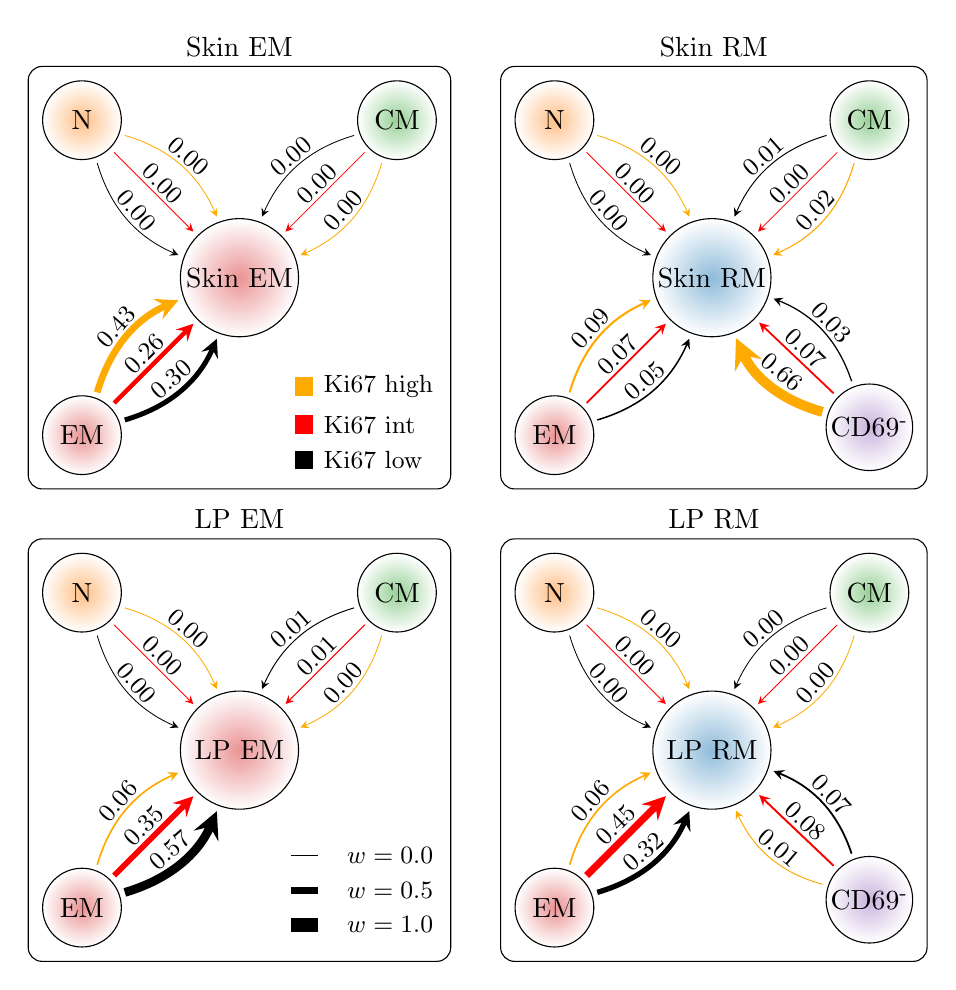
\begin{tikzpicture}
% legend for mode of entry

\matrix [below left] at (2.7, -1) {
	\node [kihinode,label=right:{\small Ki67 high}] {}; \\
	\node [kimednode,label=right:{\small Ki67 int}] {}; \\
	\node [kilonode,label=right:{\small Ki67 low}] {}; \\
};

% lewgend for the line widths

\matrix [below left, column sep = 10pt] at (2.7, -7) {
	\node (n11) {}; & \node [label=right:{\small $w = 0.0$}] (n12) {}; \\
	\node (n21) {}; & \node [label=right:{\small $w = 0.5$}] (n22) {}; \\
	\node (n31) {}; & \node [label=right:{\small $w = 1.0$}] (n32) {}; \\
};

\path (n11) edge[line width = \minw+\ewf*0] (n12);
\path (n21) edge[line width = \minw+\ewf*0.5] (n22);
\path (n31) edge[line width = \minw+\ewf*1.0] (n32); 


    \renewcommand{\wNh}{0.00}
    \renewcommand{\wCMh}{0.00}
    \renewcommand{\wEMh}{0.43}

    \renewcommand{\wNm}{0.00}
    \renewcommand{\wCMm}{0.00}
    \renewcommand{\wEMm}{0.26}

    \renewcommand{\wNl}{0.00}
    \renewcommand{\wCMl}{0.00}
    \renewcommand{\wEMl}{0.30}
    
\renewcommand{\xloc}{0.0}
\renewcommand{\yloc}{0.0}

\node[trgtnodeEM] at (0+\xloc,0+\yloc) (trgt-EM) {Skin EM};
\node[srcnodeN] at (-2+\xloc,2+\yloc) (N) {N};
\node[srcnodeCM] at (2+\xloc,2+\yloc) (CM) {CM};
\node[srcnodeEM] at (-2+\xloc,-2+\yloc) (EM) {EM};

\path[pil] (N) edge[edgekihi, line width=\minw+\ewf*\wNh] node[wbox] {\small\wNh} (trgt-EM);
\path[pil] (CM) edge[edgekihi, line width=\minw+\ewf*\wCMh] node[wbox] {\small\wCMh} (trgt-EM);
\path[pil] (EM) edge[edgekihi, line width=\minw+\ewf*\wEMh] node[wbox] {\small\wEMh} (trgt-EM);

\path[pil] (N) edge[edgekimed, line width=\minw+\ewf*\wNm] node[wbox] {\small\wNm} (trgt-EM);
\path[pil] (CM) edge[edgekimed, line width=\minw+\ewf*\wCMm] node[wbox] {\small\wCMm} (trgt-EM);
\path[pil] (EM) edge[edgekimed, line width=\minw+\ewf*\wEMm] node[wbox] {\small\wEMm} (trgt-EM);

\path[pil] (N) edge[edgekilo, line width=\minw+\ewf*\wNl] node[wbox] {\small\wNl} (trgt-EM);
\path[pil] (CM) edge[edgekilo, line width=\minw+\ewf*\wCMl] node[wbox] {\small\wCMl} (trgt-EM);
\path[pil] (EM) edge[edgekilo, line width=\minw+\ewf*\wEMl] node[wbox] {\small\wEMl} (trgt-EM);

\node[box, fit=(N)(CM)(EM)(trgt-EM), label=above:{Skin EM}] {};


    \renewcommand{\wRMh}{0.66}
    \renewcommand{\wNh}{0.00}
    \renewcommand{\wCMh}{0.02}
    \renewcommand{\wEMh}{0.09}

    \renewcommand{\wRMm}{0.07}
    \renewcommand{\wNm}{0.00}
    \renewcommand{\wCMm}{0.00}
    \renewcommand{\wEMm}{0.07}

    \renewcommand{\wRMl}{0.03}
    \renewcommand{\wNl}{0.00}
    \renewcommand{\wCMl}{0.01}
    \renewcommand{\wEMl}{0.05}
    
\renewcommand{\xloc}{6.0}
\renewcommand{\yloc}{0.0}


\node[trgtnodeRM] at (0+\xloc,0+\yloc) (trgt-RM) {Skin RM};
\node[srcnodeRMneg] at (2+\xloc,-1.9+\yloc) (CD69neg) {CD69\textsuperscript{-}};
\node[srcnodeN] at (-2+\xloc,2+\yloc) (N) {N};
\node[srcnodeCM] at (2+\xloc,2+\yloc) (CM) {CM};
\node[srcnodeEM] at (-2+\xloc,-2+\yloc) (EM) {EM};

\path[pil] (CD69neg) edge[edgekihi, line width=\minw+\ewf*\wRMh] node[wbox] {\small\wRMh} (trgt-RM);
\path[pil] (N) edge[edgekihi, line width=\minw+\ewf*\wNh] node[wbox] {\small\wNh} (trgt-RM);
\path[pil] (CM) edge[edgekihi, line width=\minw+\ewf*\wCMh] node[wbox] {\small\wCMh} (trgt-RM);
\path[pil] (EM) edge[edgekihi, line width=\minw+\ewf*\wEMh] node[wbox] {\small\wEMh} (trgt-RM);

\path[pil] (CD69neg) edge[edgekimed, line width=\minw+\ewf*\wRMm] node[wbox] {\small\wRMm} (trgt-RM);
\path[pil] (N) edge[edgekimed, line width=\minw+\ewf*\wNm] node[wbox] {\small\wNm} (trgt-RM);
\path[pil] (CM) edge[edgekimed, line width=\minw+\ewf*\wCMm] node[wbox] {\small\wCMm} (trgt-RM);
\path[pil] (EM) edge[edgekimed, line width=\minw+\ewf*\wEMm] node[wbox] {\small\wEMm} (trgt-RM);

\path[pil] (CD69neg) edge[edgekilo, line width=\minw+\ewf*\wRMl] node[wbox] {\small\wRMl} (trgt-RM);
\path[pil] (N) edge[edgekilo, line width=\minw+\ewf*\wNl] node[wbox] {\small\wNl} (trgt-RM);
\path[pil] (CM) edge[edgekilo, line width=\minw+\ewf*\wCMl] node[wbox] {\small\wCMl} (trgt-RM);
\path[pil] (EM) edge[edgekilo, line width=\minw+\ewf*\wEMl] node[wbox] {\small\wEMl} (trgt-RM);


\node[box, fit=(trgt-RM)(CD69neg)(N)(CM)(CM)(EM), label=above:{Skin RM}] {};


    \renewcommand{\wNh}{0.00}
    \renewcommand{\wCMh}{0.00}
    \renewcommand{\wEMh}{0.06}

    \renewcommand{\wNm}{0.00}
    \renewcommand{\wCMm}{0.01}
    \renewcommand{\wEMm}{0.35}

    \renewcommand{\wNl}{0.00}
    \renewcommand{\wCMl}{0.01}
    \renewcommand{\wEMl}{0.57}
    
\renewcommand{\xloc}{0.0}
\renewcommand{\yloc}{-6.0}


\node[trgtnodeEM] at (0+\xloc,0+\yloc) (trgt-EM) {LP EM};
\node[srcnodeN] at (-2+\xloc,2+\yloc) (N) {N};
\node[srcnodeCM] at (2+\xloc,2+\yloc) (CM) {CM};
\node[srcnodeEM] at (-2+\xloc,-2+\yloc) (EM) {EM};

\path[pil] (N) edge[edgekihi, line width=\minw+\ewf*\wNh] node[wbox] {\small\wNh} (trgt-EM);
\path[pil] (CM) edge[edgekihi, line width=\minw+\ewf*\wCMh] node[wbox] {\small\wCMh} (trgt-EM);
\path[pil] (EM) edge[edgekihi, line width=\minw+\ewf*\wEMh] node[wbox] {\small\wEMh} (trgt-EM);

\path[pil] (N) edge[edgekimed, line width=\minw+\ewf*\wNm] node[wbox] {\small\wNm} (trgt-EM);
\path[pil] (CM) edge[edgekimed, line width=\minw+\ewf*\wCMm] node[wbox] {\small\wCMm} (trgt-EM);
\path[pil] (EM) edge[edgekimed, line width=\minw+\ewf*\wEMm] node[wbox] {\small\wEMm} (trgt-EM);

\path[pil] (N) edge[edgekilo, line width=\minw+\ewf*\wNl] node[wbox] {\small\wNl} (trgt-EM);
\path[pil] (CM) edge[edgekilo, line width=\minw+\ewf*\wCMl] node[wbox] {\small\wCMl} (trgt-EM);
\path[pil] (EM) edge[edgekilo, line width=\minw+\ewf*\wEMl] node[wbox] {\small\wEMl} (trgt-EM);

\node[box, fit=(N)(CM)(EM)(trgt-EM), label=above:{LP EM}] {};


    \renewcommand{\wRMh}{0.01}
    \renewcommand{\wNh}{0.00}
    \renewcommand{\wCMh}{0.00}
    \renewcommand{\wEMh}{0.06}

    \renewcommand{\wRMm}{0.08}
    \renewcommand{\wNm}{0.00}
    \renewcommand{\wCMm}{0.00}
    \renewcommand{\wEMm}{0.45}

    \renewcommand{\wRMl}{0.07}
    \renewcommand{\wNl}{0.00}
    \renewcommand{\wCMl}{0.00}
    \renewcommand{\wEMl}{0.32}
    
\renewcommand{\xloc}{6.0}
\renewcommand{\yloc}{-6.0}


\node[trgtnodeRM] at (0+\xloc,0+\yloc) (trgt-RM) {LP RM};
\node[srcnodeRMneg] at (2+\xloc,-1.9+\yloc) (CD69neg) {CD69\textsuperscript{-}};
\node[srcnodeN] at (-2+\xloc,2+\yloc) (N) {N};
\node[srcnodeCM] at (2+\xloc,2+\yloc) (CM) {CM};
\node[srcnodeEM] at (-2+\xloc,-2+\yloc) (EM) {EM};

\path[pil] (CD69neg) edge[edgekihi, line width=\minw+\ewf*\wRMh] node[wbox] {\small\wRMh} (trgt-RM);
\path[pil] (N) edge[edgekihi, line width=\minw+\ewf*\wNh] node[wbox] {\small\wNh} (trgt-RM);
\path[pil] (CM) edge[edgekihi, line width=\minw+\ewf*\wCMh] node[wbox] {\small\wCMh} (trgt-RM);
\path[pil] (EM) edge[edgekihi, line width=\minw+\ewf*\wEMh] node[wbox] {\small\wEMh} (trgt-RM);

\path[pil] (CD69neg) edge[edgekimed, line width=\minw+\ewf*\wRMm] node[wbox] {\small\wRMm} (trgt-RM);
\path[pil] (N) edge[edgekimed, line width=\minw+\ewf*\wNm] node[wbox] {\small\wNm} (trgt-RM);
\path[pil] (CM) edge[edgekimed, line width=\minw+\ewf*\wCMm] node[wbox] {\small\wCMm} (trgt-RM);
\path[pil] (EM) edge[edgekimed, line width=\minw+\ewf*\wEMm] node[wbox] {\small\wEMm} (trgt-RM);

\path[pil] (CD69neg) edge[edgekilo, line width=\minw+\ewf*\wRMl] node[wbox] {\small\wRMl} (trgt-RM);
\path[pil] (N) edge[edgekilo, line width=\minw+\ewf*\wNl] node[wbox] {\small\wNl} (trgt-RM);
\path[pil] (CM) edge[edgekilo, line width=\minw+\ewf*\wCMl] node[wbox] {\small\wCMl} (trgt-RM);
\path[pil] (EM) edge[edgekilo, line width=\minw+\ewf*\wEMl] node[wbox] {\small\wEMl} (trgt-RM);


\node[box, fit=(trgt-RM)(CD69neg)(N)(CM)(CM)(EM), label=above:{LP RM}] {};

\end{tikzpicture}
\end{document}
